%BEGIN_FOLD
% !TeX document-id = {7ed1036c-f6fe-486f-b58e-dfc79e34db3a}
% !TeX TXS-program:compile = txs:///pdflatex/[--shell-escape]

\documentclass[inzynier,druk]{dyplom}
%\documentclass[magister,archiwum]{dyplom}

\usepackage[utf8]{inputenc}
\usepackage{hyperref}
\usepackage[toc]{appendix}
\renewcommand{\appendixtocname}{Dodatki}
\renewcommand{\appendixpagename}{Dodatki}

% pakiet do składu listingów 
% w razie potrzeby można odblokować możliwość numerowania linii
% lub zmienić wielkość czcionki w listingu
\usepackage{minted}
\setminted{breaklines,
frame=lines,
framesep=5mm,
baselinestretch=1.1,
fontsize=\small,
%linenos
}

% nowe otoczenie do składania listingów
\usepackage{float}
\newfloat{listing}{htp}{lop}
\floatname{listing}{Listing}
\usepackage{chngcntr}
\counterwithin{listing}{chapter}

% patch wyrównujący spis listingów do lewego marginesu 
%https://tex.stackexchange.com/questions/58469/why-are-listof-and-listoffigures-styled-differently
\makeatletter
\renewcommand*{\listof}[2]{%
  \@ifundefined{ext@#1}{\float@error{#1}}{%
    \expandafter\let\csname l@#1\endcsname \l@figure  % <- use layout of figure
    \float@listhead{#2}%
    \begingroup
      \setlength\parskip{0pt plus 1pt}%               % <- or drop this line completely
      \@starttoc{\@nameuse{ext@#1}}%
    \endgroup}}
\makeatother

\usepackage{url}
\usepackage{amssymb}

%END_FOLD

% Dane o pracy (strona tytułowa)
\author{Mateusz Gawłowski}
\title{Projekt i implementacja modułu ekstrakcji podsumowań danych w systemie autonomicznym}
\titlen{Design and implementation of a module for extraction of data summaries by an autonomus system}
\promotor{dr hab. inż. Radosław Katarzyniak, prof. PWr}
\wydzial{Wydział Informatyki i Zarządzania}
\kierunek{Informatyka}
\krotkiestreszczenie{W pracy przedstawiono projekt oraz implementację modułu ekstrakcji podsumowań danych w gotowej aplikacji programowego agenta rozwiązującego zadanie generowania podsumowań lingwistycznych w postaci modalnych zdań reprezentujących wiedzę agenta o stanie obiektu ulokowanego w świecie rzeczywistym. Przedstawiono przykład działania agenta.}
\slowakluczowe{agent wbudowany,	agent kognitywny, pamięć semantyczna, ekstrakcja podsumowań danych}

\begin{document}

\maketitle

\pagenumbering{gobble}
\tableofcontents

\pagenumbering{arabic}
\chapter*{Streszczenie}
\setcounter{page}{3}

Celem pracy było opracowanie modułu ekstrakcji podsumowań danych w autonomicznym systemie agentowym. Rozwiązania zawarte w obecnym module mają duży margines poprawy, a zmiany w dużym stopniu wpłyną na jakość i wydajność agenta. W ramach pracy przygotowano nowy moduł, w którym opracowano nowe sposoby generowania i~aktualizacji podsumowań. Oprócz projektu aplikacji praca zawiera wyniki testów ukazujące wpływ zaproponowanego rozwiązania na wydajność. Przygotowana w ramach projektu inżynierskiego praca może służyć do różnego rodzaju badań oraz być dalej rozwijana.


\addtocontents{toc}{\protect\setcounter{tocdepth}{-1}}
\begingroup
\renewcommand{\cleardoublepage}{}
\renewcommand{\clearpage}{}
\chapter*{Abstract}

The purpose of the thesis was to develop a module for extracting data summaries in an autonomous agent system. Solutions included in the current module have a large margin of improvement, and changes will greatly affect the quality and efficiency of the agent. As part of the thesis, a new module was prepared in which new ways of generating and updating summaries were developed. In addition to the application design, the thesis contains test results showing the impact of the proposed solution on the performance. The thesis prepared as part of the engineering project can be used for various types of research and be further developed.


\endgroup
\addtocontents{toc}{\protect\setcounter{tocdepth}{2}}
% --- Koniec strony ze streszczeniem i abstraktem -----------------------------------------------------------

\chapter*{Wstęp}

<tekst>


\section*{Opis problemu}

<tekst>


\section*{Cel i zakres pracy}

<tekst>


\section*{Treść pracy}

<tekst>


\chapter{Podstawy teoretyczne w zakresie tematyki pracy}

Tematyka pracy dotyczy dziedziny, która w literaturze określana jest terminem obliczeń kognitywnych (ang. \textit{cognitive computing}). Obejmuje ona inteligentne modele i metody obliczeniowe, które wyznaczają kierunek dalszego rozwoju systemów tak zwanych inteligencji wbudowanej oraz środowisk inteligentnych \cite{hur15}.

Podstawą wspomnianej dziedziny jest upodabnianie funkcjonowania oprogramowania lub sprzętu do działania ludzkiego mózgu. Współczesne rozwiązania (takie jak  Watson \cite{kel13}) korzystają z wielu zaawansowanych narzędzi do analizy i przetwarzania danych --- między innymi uczenie maszynowe, przetwarzanie języka naturalnego. Symulują w ten sposób działanie mózgu w oparciu o duże zbiory danych, by w przyszłości podejmować nawet istotne decyzje medyczne \cite{woo15}. Takie podejście ignoruje jednak poznawczą naturę działania mózgu, skupiając się przede wszystkim na satysfakcjonujących rezultatach, a nie próbach wiernego oddaniu sposobu w jaki funkcjonuje mózg, procesów myślowych i poznawczych.

W odróżnieniu od wspomnianego podejścia rozwiązania zastosowane w aplikacji należą do obszaru określanego jako lingwistyka kognitywna. Tym samym pozostają w większym stopniu związane z pojęciem kognitywistyki samym w sobie. Jest to interdyscyplinarna dziedzina nauki z pogranicza między innymi filozofii, psychologii, sztucznej inteligencji i lingwistyki (określana także jako nauki kognitywne, poznawcze). Dotyczy ona obserwacji i analizy działania zmysłów, mózgu i umysłu oraz ich modelowania \cite{tha17}.

W pracy, a także w całej aplikacji zaproponowana została oryginalna semantyka kognitywna. Pozostaje ona w zgodzie z ogólnie przyjętymi teoriami modalnego języka komunikacji \cite{tal00}, będących częścią lingwistyki kognitywnej. Zaproponowana implementacja systemu kognitywnego agenta jest w ścisłej relacji z formalną teorią kognitywną zaprezentowaną w \cite{kat07}. Zauważa się jednak brak publikacji bezpośrednio powiązanych z realizowanym systemem agentowym.

W dalszej części tego rozdziału zawarto podstawowe wprowadzenie teoretyczne przybliżające zagadnienia i modele, na których opiera się aplikacja agenta oraz opracowany moduł zarządzania pamięcią semantyczną. Przedstawiono przede wszystkim te elementy projektowanego systemu agentowego (agenta i jego otoczenia), które są bezpośrednio powiązane z nowym modułem: model zewnętrznego względem agenta świata rzeczywistego i objętego jego działaniem obserwacyjnym, model enkapsulowanej (prywatnej) epizodycznej bazy wiedzy służącej do przechowywania pojedynczych obserwacji świata zewnętrznego oraz model semantycznej wiedzy agenta opartej na koncepcji holonów, jako oryginalne rozszerzenie reprezentujące wynik ekstrakcji podsumowań danych.

Szczegółowy opis wszystkich zagadnień i poszczególnych składowych opracowanego modelu można znaleźć w raporcie dotyczącym wspomnianej aplikacji \cite{raport}. Większość przyjętych założeń funkcjonalnych wprowadzona została we wcześniejszych pracach dotyczących przetwarzania modalnych języków komunikacji --- np. \cite{kat07} \cite{kat99}.


\section{Model świata rzeczywistego}

Zewnętrznym światem rzeczywistym \textit{S} projektowanego agenta jest dla niego otoczenie, w którym został umieszczony, i który objęty jest przez niego aktywnością obserwacyjną. Głównym elementem świata oraz przedmiotem obserwacji są obiekty umieszczone w świecie \textit{S}. Dalej omówione zostały poszczególne elementy modelu.


	\subsection{Obiekty}
	
	Świat \textit{S} zbudowany jest z atomowych obiektów, --- są to proste obiekty, dla których możliwe jest zdefiniowanie zbioru cech jakimi się charakteryzują. Ograniczenie modelu wyłącznie do obiektów atomowych, w przeciwieństwie do świata, który naprawdę składa się z krotek obiektów atomowych, które reprezentują obiekty złożone wynika z założeń przyjętych w projekcie. Dzięki temu uproszczeniu wyeliminowane zostały wszelkie zależności między obiektami co w znaczącym stopniu zawęża przestrzeń rozważań.
	
	
	\subsection{Klasy obiektów}
	
	Obiekty atomowe świata pogrupowane zostały w klasy 
	\textit{N\textsubscript{i(i=1,2,...,Q)}}. 
	Każdy potencjalny --- obserwowalny przez agenta --- obiekt umieszczony w świecie \textit{S} przynależy do jednej z klas
	\textit{N\textsubscript{i}}. 
	Pełnić będą one rolę tak zwanych nośników systemów relacyjnych oraz są predefiniowane w systemie projektowanego agenta. Relacje definiują atomowe cechy, którymi charakteryzują się obiekty danej klasy 
	\textit{N\textsubscript{i}}. 
	Właśnie z takich nośników zbudowane będą potencjalne stany rzeczywistego świata zewnętrznego. Klasa definiuje zatem wszystkie możliwe zbiory relacyjne, którymi można opisać obiekt należący do tejże klasy.
	
	
	\subsection{Stan świata}
	
	W przyjętym modelu każdy z zaobserwowanych przez agenta stanów świata rzeczywistego \textit{S} ma przypisany odpowiadający mu moment w czasie 
	\textit{t\textsuperscript{ S} ∈ T\textsuperscript{ S}}. 
	We wszystkich punktach 
	\textit{t\textsuperscript{ S} ∈ T\textsuperscript{ S}} 
	stan świata składa się z atomowych obiektów doświadczonych przez agenta w danym czasie 
	\textit{t\textsuperscript{ S}}.
	Obiekty reprezentowane są przez listy cech (zgodnych z ich przynależnością do klas 
	\textit{N\textsubscript{i}}), 
	które z punktu widzenia agenta obiekt posiadał w punkcie 
	\textit{t\textsuperscript{ S} ∈ T\textsuperscript{ S}}.
	Ważnym założeniem przyjętym przy realizacji projektu jest to, że ogląd świata wykonany przez agenta może być różny od stanu faktycznego, w jakim ten świat się znajdował.
	
	% chronologia
	
	Punkty zbioru 
	\textit{T\textsuperscript{ S}} 
	określają porządek chronologiczny wśród zaobserwowanych stanów świata rzeczywistego. Wyznaczane są one arbitralnie przez agenta w oparciu o zegar globalny. Agent sam podejmuje decyzje kiedy kończy ogląd świata w danym 
	\textit{t\textsuperscript{ S}\textsubscript{i}}, 
	a kolejnemu przypisany zostanie punkt (moment)
	\textit{t\textsuperscript{ S}\textsubscript{i+1}}.
	Wykorzystany czas globalny jest więc jedynie pozorną miarą, która nie ma związku z rzeczywistym upływem czasu, a służy jedynie zachowaniu liniowego porządku chronologicznego.
	
	
	\subsection{Cechy i opis świata}
	
	Opis stanu świata zbudowany jest z obiektów, opisanych za pomocą zestawów predefiniowanych cech 
	\textit{P\textsubscript{i(i=1,2,...,K)}}, 
	pochodzących z klas 
	\textit{N\textsubscript{i}} 
	do których należą poszczególne obiekty. Cechy są atomowe --- zauważyć można jedynie obecność lub brak danej cechy w danym obiekcie. Posiadanie lub nie posiadanie konkretnej cechy
	\textit{P\textsubscript{i}}
	przez rzeczywisty obiekt atomowy w punkcie (momencie) czasu
	\textit{t\textsuperscript{ S} ∈ T\textsuperscript{ S}} 
	reprezentowane jest przez obecność tego obiektu w odpowiednich relacjach przedstawiających rozkłady cech w obiektach. Przyjęte zostało założenie, że lista cech przypisywanych obiektom nie zmienia się --- jest stała. 

	Założono, że narzędzia percepcyjne docelowego agenta umożliwiać będą zidentyfikowanie przynależność obiektu do danej klasy oraz bezpośrednią obserwację stanów tych cech w obiektach rzeczywistych. Zgodnie 
	z wcześniejszym założeniem o możliwych różnicach między stanem świata postrzeganym przez agenta, a stanem faktycznym, zakłada się również, że w pewnych warunkach niezależących od agenta (np. niedostatecznego oświetlenia) stan cechy nie tylko może zostać błędnie ustalony, ale też stwierdzenie stanu tej cechy jest niemożliwe. Biorąc powyższe założenia pod uwagę pojedyncza cecha danego obiektu może mieć trzy stany: 

	\begin{itemize}
	 	\setlength{\itemindent}{.5in}
		\item zaobserwowano występowanie cechy \textit{P\textsubscript{i}},
		\item zaobserwowano brak cechy \textit{P\textsubscript{i}},
		\item niemożliwe jest określenie stanu cechy
			\textit{P\textsubscript{i}}.
	\end{itemize}
	
	Uporządkowane liniowo obserwacje stanu świata stanowią jedyne źródło subiektywnej wiedzy empirycznej (wiedzy opartej na doświadczeniu) agenta na temat świata. Wszelki brak wiedzy na temat cech obiektów w najnowszym (bieżącym) zaobserwowanym stanie świata, zostanie uzupełniony przez wbudowane procesy kognitywne. Tym samym wiedza agenta o stanie świata nie jest tożsama z jego wiedzą o bieżącym stanie świata.
	
	Kluczowym zadaniem realizowanego agenta jest wyrażenie treści subiektywnych przekonań na temat świata w sytuacji, gdy przeprowadzenie kompletnego oglądu, z różnych powodów, nie będzie możliwe.
	

\section{Model epizodycznej bazy wiedzy}

Epizodyczna baza wiedzy jest enkapsulowaną w agencie prywatną bazą, stanowiącą podstawowy reprezentację wiedzy przechowywanej przez agenta na temat stanu zewnętrznego świata rzeczywistego. W dowolnym globalnym punkcie 
\textit{t\textsuperscript{ S}} 
zawiera tylko te obiekty, o których istnieniu fizycznym agent jest przekonany w punkcie 
\textit{t\textsuperscript{ S}}.

Baza zbudowana jest z uporządkowanych liniowo w czasie epizodów. Wiedza agenta w punkcie \textit{t}, składa się ze zbioru wszystkich epizodów e, dla których spełniona jest zależność \textit{t\textsubscript{e} ≤ t}.

Epizod dotyczący punktu w czasie \textit{t} składa się z relacji \textit{P\textsuperscript{ +}\textsubscript{i}} 
oraz 
\textit{P\textsuperscript{ --}\textsubscript{i}}, 
które mówią odpowiednio o występowaniu (+) lub niewystępowaniu (--) cechy
\textit{P\textsubscript{i}}. 
Te zbiory wypełnione są obiektami, u których agent w czasie \textit{t} stwierdził obecność lub brak \textit{i}-tej cechy \textit{P}. Obiekty mogą być przypisane tylko do cech zgodnych z klasą, do której należą. 

Dodatkowym założeniem jest to, że brak obiektu w zbiorach 
\textit{P\textsuperscript{ +}\textsubscript{i}} i 
\textit{P\textsuperscript{ --}\textsubscript{i}},  
rozumiane jest jako sytuacja, w której agent nie był w stanie określić stanu cechy 
\textit{P\textsubscript{i}} 
podczas oglądu świata w danym epizodzie.

Istotną kwestią jest wymóg zachowania rozłączności wyżej wspomnianych zbiorów --- 
\textit{P\textsuperscript{ +}\textsubscript{i}(t) ⋂ P\textsuperscript{ --}\textsubscript{i}(t) = ⊘} 
dla każdego \textit{i} oraz \textit{t}. Warunek ten jest obligatoryjny, gdyż nie spełnienie go prowadzi do sprzeczności w zasobach wiedzy agenta.

\section{Model semantycznej bazy wiedzy}




%%%%%%%%%%%%%%%%%%%%%%%%%%%%%%%%%%

%pozostają w ścisłej relacji z oryginalnymi teoriami modalnego języka komunikacji, opisującymi zasady poprawnej i zdroworozsądkowo akceptowanej implementacji w interaktywnych systemach komputerowych tzw. kognitywnych semantyk modalnych zdań autoepistemicznych. Teorie te przynależą do obszaru (stosowanej) lingwistyki kognitywnej [Lak87] [Tal00] i jako przypadek szczególny obejmują modalne rozszerzenia zdań prostych stwierdzających wystąpienie albo brak wystąpienia cechy w konkretnym obiekcie, jak też dwuczłonowych koniunkcji, dwuczłonowych alternatyw włączających i dwuczłonowych alternatyw wykluczających złożonych ze zdań prostych [Kat07]. Sygnalizowane teorie semantyk kognitywnych formułują m.in. szczegółowe dezyderaty co do adekwatnej organizacji i treści baz wiedzy obligatoryjnie uczestniczących w realizacji procesów generowania wymienionej klasy zdań (traktowanych jako odpowiedzi na zapytania). Założenia strukturalne i funkcjonalne formułowane w teoriach semantyki kognitywnej odzwierciedlone zostały w architekturze, projekcie i implementacji agenta powstającego w ramach niniejszego projektu.

%Proponowana implementacja pozostaje w ścisłej relacji z akceptowanym powszechnie przepływowym (ang. pipeline) modelem generowania zdań języka naturalnego [Wan16] [Wal02] [Ram16] [Mel06] wnosząc jednocześnie elementy oryginalne specyficzne dla formalnej teorii kognitywnej prezentowanej m.in. w [Kat07].

%%%%%%%%%%%%%%%%%%%%%%%%%%%%%%%%%%
\chapter{Założenia projektowe}

Ten rozdział posłuży przybliżeniu działania zrealizowanej aplikacji agenta od strony praktycznej oraz przedstawienie założeń przyjętych dla opracowanego rozszerzenia. 

Opisane zostaną najważniejsze, zaimplementowane w systemie funkcjonalności. Opis ten będzie kluczowy w zrozumieniu założeń projektowych rozszerzenia oraz ich wagę dla usprawnienia działania agenta. Oprócz tego przedstawiony zostanie prosty przykład pracy agenta, co zilustruje poszczególne etapy jego pracy. Dalej wskazano problem z jakim zmierzono się w tej pracy, poprzez ukazanie elementów, które na tle całej aplikacji wymagają usprawnienia. Na końcu sformułowano wymagania funkcjonalne i niefunkcjonalne dla nowego modułu ekstrakcji podsumowań danych.


\section{Opis aplikacji bazowej}

Poniżej przybliżona została architektura i funkcjonalności aplikacji nazwanej \textit{ModalCommLangGrounding}, która  w ramach tej pracy jest rozszerzana. Poszczególne elementy tego systemu widoczne są na rysunku \ref{rys:schemat}. Aplikacja została ona opracowana w modelu obiektowym i realizuje, w warstwie oprogramowania, system wbudowanego agenta. Do implementacji wykorzystano język programowania \textit{Java} w wersji \textit{1.8}.

Aplikacja realizuje przetwarzanie obserwacji, zawierających informacje o fizycznych stanach cech obiektu. Umożliwia to generowanie na ich podstawie podsumowań lingwistycznych w języku naturalnym na temat aktualnego stanu obiektów. Obserwacje przechowywane są w odpowiednio przygotowanej bazie danych, która w obrębie działającego agenta jest wypełniana poprzez zewnętrzne mechanizmy. Do realizacji bazy danych wykorzystano bibliotekę \textit{SQLite} implementującą prosty silnik SQL. Technologia \textit{SQLite} nie wymaga do działania osobnego procesu zarządzania relacyjną bazą danych, dlatego jest optymalnym rozwiązaniem dla realizowanego agenta i innych systemów wbudowanych.

\begin{figure}  
	\centering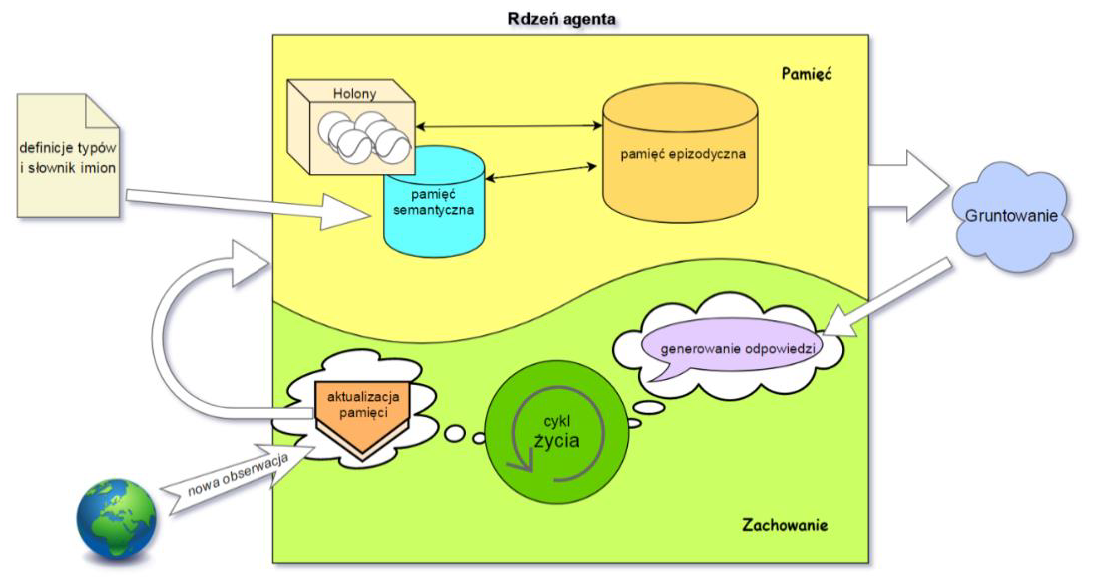
\includegraphics[width=.9\textwidth]{img/agent-schemat}
	\caption{Koncepcyjny schemat aplikacji agenta \cite{raport}}
	\label{rys:schemat}
\end{figure}

Model świata (otoczenie) w którym umieszczony został potencjalny agent jest w pełni deterministyczny. Wszystkie możliwe do zaobserwowania typy obiektów, jak również ich zestawy cech są predefiniowane przez użytkownika w pliku konfiguracyjnym w formacie XML. Te informacje są podstawowym elementem wiedzy semantycznej agenta oraz stanowi źródło struktury danych w bazie, do której dodawane są obserwacje. Zdolność do zaobserwowania cech obiektu jest w pełni uzależniona od definicji jego typu (klasy). Oprócz tego częścią wiedzy semantycznej jest również zbiór rozpoznanych obiektów. Do parsowania plików XML wykorzystano bibliotekę \textit{XStream}.

Każdy obiekt umieszczony w świecie agenta musi zawierać identyfikator, aby mógł zostać rozpoznany, np.\ kod kreskowy (przygotowano mechanizm pozwalający na używanie wielu rodzajów identyfikatorów jednocześnie). Użycie identyfikatorów umożliwia agentowi rozróżnianie poszczególnych obiektów. Dodatkowo część identyfikatora określa jego przynależność do danego typu obiektów. Pozwala to na poznanie zestawu potencjalnych cech, których występowanie w tym obiekcie powinno zostać przez agenta rozpoznane. 

Obserwacja w tak skonstruowanym modelu reprezentowana jest jako pojedyncze doświadczenie stanu obiektu. Stan jako doświadczenie epizodyczne jest zestawem zaobserwowanych cech. Pojedyncza cecha jest atomowa, a jej wartość informuje o tym czy w~danym obiekcie stwierdzono obecność, brak lub niemożność określenia występowania tej cechy. Przykładem takiej cechy jest \textit{zielony kolor}. Wartość tej cechy w danej obserwacji interpretowana jest w taki sposób, że  obiekt o identyfikatorze $ id $ w momencie $ t $ jest koloru zielonego, nie jest koloru zielonego lub nie stwierdzono czy jest koloru zielonego.

Tak zdefiniowana obserwacja wraz z identyfikatorem konkretnego obiektu oraz znacznikiem czasu przechowywane są w fizycznej bazie SQL agenta, która stanowi jedyne źródło wiedzy empirycznej agenta. Zakłada się, że agent wyposażony jest w odpowiednie narzędzia percepcyjne, którymi dokonuje oglądu obiektów umieszczonych w jego zewnętrznym świecie rzeczywistym. Realizowana aplikacja korzysta już z wypełnionej (oraz reaguje na nowe obserwacje) bazy danych i nie zawiera mechanizmów percepcyjnych.

Za pomocą obserwacji pobranych z bazy, pogrupowanych według znacznika czasu, tworzone są tak zwane epizody. Dany epizod dotyczy konkretnego punktu w czasie i~zawiera zbiory obiektów, dla których zaobserwowano że występuje, nie występuje lub nie stwierdzono czy występuje każda z cech. Kolekcja epizodów stanowi podstawowe źródło wiedzy empirycznej agenta i jest częścią jego pamięci (rys. \ref{rys:schemat}). Za bieżący stan świata uznawany jest epizod o najwyższym znaczniku czasu.

Na podstawie zebranej wiedzy agentowi może zostać zadane przez użytkownika pytanie na temat aktualnego stanu konkretnego obiektu. Może ono dotyczyć występowania albo braku występowania pojedynczej cechy lub kilku cech w formie dwuczłonowej koniunkcji. Odpowiedzią agenta jest modalne zdanie języka naturalnego zawierające subiektywne przekonanie na temat bieżącego stanu podanych cech. Agent po otrzymaniu zapytania upewnia się, czy stan jego wiedzy epizodycznej jest aktualny, tzn. czy w bazie danych nie ma obserwacji, które najpierw powinny zostać wczytane do jego pamięci epizodycznej.

W przypadku, gdy wiedza o aktualnym stanie świata jest niewystarczająco kompletna, to znaczy gdy występowanie cechy zawartej w pytaniu nie zostało z różnych powodów określone (np.\ niedostateczne oświetlenie), agent w oparciu o wiedzę dotyczącą wcześniejszych stanów obiektu dokonuje gruntowania wiedzy. Dotyczy to zarówno pytania o jedną cechę, jak i o dwie cechy w przypadku gdy przynajmniej jedna z nich jest nieokreślona. Efektem końcowym jest odpowiedź o odpowiednim stopniu modalności z użyciem operatorów: 

\begin{itemize}
	\setlength{\itemindent}{.5in}
	\item "Możliwe, że (...)" -- operator \textit{POS},
	\item "Sądzę, że (...)" -- operator \textit{BEL},
	\item "Wiem, że (...)" -- operator \textit{KNOW}.
\end{itemize}  

Przy czym to, który z nich zostanie użyty zależy od stopnia przekonania agenta oraz zdefiniowanych przez użytkownika progów modalności. Innymi słowy są to granice, które wyznaczają moment w którym agent interpretuje swoją wiedzę z mniejszym lub większym przekonaniem co do zgodności z rzeczywistością. Wpływ na to ma względna liczność poszczególnych zbiorów epizodów, reprezentujących relewantne doświadczenia z przeszłości (odnoszące się do danego obiektu i cech). Częstsze występowanie danej predykacji skutkuje silniejszymi przekonaniami agenta o możliwości jej wystąpienia w rzeczywistości.

Strukturą wiedzy łączącą powiązane ze sobą i logicznie dopełniające się zbiory gruntujące jest holon. Zbiór holonów przynależy do wiedzy semantycznej agenta. Utworzone podczas gruntowania wiedzy holony przechowywane są w odpowiedniej kolekcji. Holon, jeśli jest aktualny, może zostać ponownie wykorzystany do bezpośredniego skonstruowania zdania modalnego na temat obiektu oraz cech, których dotyczy. W przypadku, gdy nie jest aktualny, to w pierwotnej wersji aplikacji holon ten budowany jest od nowa. Rozróżniane są holony proste dotyczące jednej cechy oraz holony złożone dotyczące współwystępowania dwóch cech. Zgodnie z rysunkiem \ref{rys:holony} przechowują one odpowiednio dwie i cztery wartości reprezentujące wszystkie kombinacje występowania cech $ p $ i $ q $.

\begin{figure}  
	\centering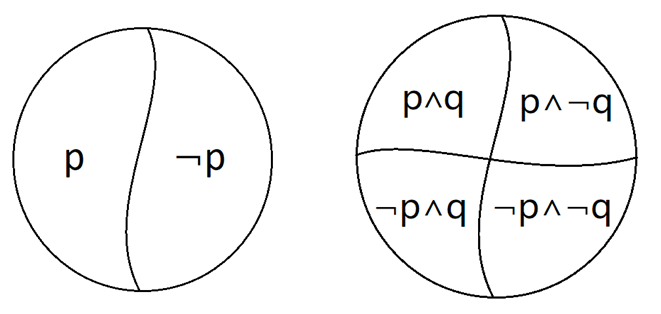
\includegraphics[width=.6\textwidth]{img/holony}
	\caption{Budowa holonu prostego (po lewej) i złożonego (po prawej)}
	\label{rys:holony}
\end{figure}

Aplikację agenta uruchomić można w trybie programowym. Przygotowany został do tego mechanizm przeprowadzania symulacji z użyciem plików w formacie CSV. Pozwala to na sprawne wczytanie do wiedzy agenta informacji o obiektach oraz obserwacji. Dodatkowo używając tego samego pliku po każdej wczytanej obserwacji mogą zostać sformułowane zapytania do agenta dotyczące stanu wiedzy po danej obserwacji. Pozwala to na prześledzenie zmian w przekonaniach agenta pod wpływem kolejnych obserwacji obiektów. Dodatkowo możliwe jest też ręczne wprowadzanie nowych obserwacji do bazy danych (pozwalają na to narzędzia niektórych środowisk programistycznych) oraz zadawanie pytań poprzez linię komend w trakcie działania agenta. 

Jednakże docelowym trybem pracy agenta jest praca w czasie rzeczywistym oparta na wielowątkowości. Cykl życia agenta (widoczny na rysunku \ref{rys:schemat}) pozwala mu na samodzielne aktualizowanie stanu jego wiedzy oraz komunikację głosową z użytkownikiem końcowym (głównie człowiekiem). Wątek aktualizacji uruchamiany jest tylko w sytuacji bezczynności --- braku aktywnej komunikacji. Do rozpoznawania mowy wykorzystano odrębny, zewnętrzny moduł, który zaimplementowany został w języku C\# z wykorzystaniem platformy \textit{Microsoft.Speech} oraz pliku gramatyki w formacie XML, który zawiera predefiniowane nazwy cech oraz obiektów, co umożliwia rozpoznanie poszczególnych wyrazów. Agent nasłuchuje zdań, które mogą zostać przetworzone i na ich podstawie generowane są podsumowania lingwistyczne. Przyjęte zdania tworzą tak zwaną kolejkę FIFO (First In, First Out), gdzie rozpatrywane są w kolejności z jaką się pojawiły. Wygenerowane podsumowanie przesyłane jest z powrotem do modułu komunikacji, który syntezuje głosową odpowiedź i~wypowiada ją do użytkownika.


\section{Przykład pracy agenta}

Poniżej przedstawiono przykładowy scenariusz pracy agenta. Został on odpowiednio uproszczony, tak aby przedstawić przede wszystkim kolejne etapy pracy agenta oraz podkreślić zmienność jego przekonań o stanie świata rzeczywistego (obiektów w nim umieszczonych). Przykład opracowano na podstawie \cite{kat17}, gdzie również zaprezentowane zostały scenariusze ekstrakcji podsumowań lingwistycznych.

Założono, że w otoczeniu agenta są tylko dwa obiekty o identyfikatorach 1101 i 1102. Są one tego samego typu, co jest dedukowane na podstawie dwóch pierwszych cyfr identyfikatora. W języku naturalnym będą nazywane odpowiednio \textit{Foobar} i \textit{Foobaz}. Obiekty typu 11 (reprezentującym np.\ piłki) charakteryzują się dwiema cechami --- mogą być okrągłe i/lub kolorowe. Każda cecha może mieć trzy stany, które oznaczone są w następujący sposób:

\begin{enumerate}
	\setlength{\itemindent}{.5in}
	\item \hspace{.05in} "$+$" - cecha występuje w obiekcie,
	\item \hspace{.05in} "$-$" - brak cechy w obiekcie,
	\item \hspace{.05in} "$?$" $\space$ - nie udało się określić stanu cechy.
\end{enumerate}  

Agent w momencie uruchomienia ma pustą pamięć, jednakże w źródłowej bazie danych mogą być już obecne obserwacje. Cykl życie agenta wykonuje okresowo dwie czynności: sprawdza czy w bazie nie ma nowych obserwacji, z których powinny zostać zbudowane epizody oraz czy w kolejce pytań jest zdanie, które oczekuje na przetworzenie. W tym przykładzie baza danych, w momencie uruchomienia, ma już przeprowadzonych sześć obserwacji, które przedstawiono w tabeli \ref{tab:obserwacje1}. Agent buduje z nich odpowiednie epizody, które ładuje do pamięci epizodycznej.

\begin{table}[H]
	\caption{Obserwacje obecne w bazie danych przed uruchomieniem agenta}
	\label{tab:obserwacje1}
	\centering
	\begin{tabular}{|l|l|c|c|} \hline
		\textbf{Czas} & \textbf{Identyfikator} & \textbf{Okrągły} & \textbf{Kolorowy} \\ \hline
		1  &  1101  &  $ + $  &  $ + $  \\ \hline
		1  &  1102  &  $ + $  &  $ - $  \\ \hline
		2  &  1101  &  $ + $  &  $ - $  \\ \hline
		2  &  1102  &  $ + $  &  $ - $  \\ \hline
		3  &  1101  &  $ + $  &  $ ? $  \\ \hline
		3  &  1102  &  $ + $  &  $ + $  \\ \hline
	\end{tabular}
\end{table}

Podstawowa wiedza agenta zbudowana jest z epizodów, wykorzystywane są one do gruntowania przekonań agenta. Pojedynczy epizod przechowuje następujące informacje: znacznik czasu oraz zbiory cech występujących, niewystępujących oraz nieokreślonych (wraz z listami obiektów). Zgodnie z tą strukturą trzeci epizod ma następującą postać:

\begin{itemize}
	\setlength{\itemindent}{.5in}
	\item znacznik czasu $ = $ 3,
	\item cechy występujące $ = $ \{ \{Okrągły, \{1101, 1102\}\}, \{Kolorowy, \{1102\}\} \},
	\item cechy niewystępujące $ = $ \{ \},
	\item cechy nieokreślone $ = $ \{ \{Kolorowy, \{1101\}\} \}.
\end{itemize}  

Użytkownik zadaje następujące pytanie agentowi: "Czy Foobar jest okrągły?". Pierwszą czynnością wykonywaną przez agenta jest zawsze sprawdzenie czy stan jego wiedzy jest aktualny. Innymi słowy, czy w bazie danych są obserwacje, które nie zostały jeszcze wprowadzone do pamięci. Jeśli tak, agent najpierw przeprowadza aktualizację. W kolejnym kroku przeszukiwana jest wiedza agenta o bieżącym (najnowszym) stanie świata. W tym przypadku pozwala ona otrzymać bezpośrednią odpowiedź na zadane pytanie -- trzeci epizod (przedstawiony wcześniej) zawiera informacje o tym, że w obiekcie 1101 (nazwanym Foobar) występuje cecha "okrągły". Dzięki temu agent może od razu udzielić odpowiedź: "Wiem, że Foobar jest okrągły.".

Zanim użytkownik zada kolejne pytania, agent dwukrotnie dokonuje oglądu otoczenia. Nowe obserwacje (przedstawione w tabeli \ref{tab:obserwacje2}) wczytywane są do epizodycznej pamięci agenta. 

\begin{table}[H]
	\caption{Nowe obserwacje w źródłowej bazie danych}
	\label{tab:obserwacje2}
	\centering
	\begin{tabular}{|l|l|c|c|} \hline
		\textbf{Czas} & \textbf{Identyfikator} & \textbf{Okrągły} & \textbf{Kolorowy} \\ \hline
		4  &  1101  &  $ - $  &  $ - $  \\ \hline
		4  &  1102  &  $ + $  &  $ - $  \\ \hline
		5  &  1102  &  $ - $  &  $ ? $  \\ \hline
	\end{tabular}
\end{table}

Użytkownik powtarza pytanie zadane wcześniej, które brzmiało: "Czy Foobar jest okrągły?". Tym razem sytuacja jest inna -- agent nie posiada żadnej wiedzy na temat bieżącego stanu tego obiektu. Nie istnieje też aktualny holon, który jest adekwatny do zadanego pytania. Tym samym agent zmuszony jest uzupełnić swoje przekonania procesem gruntowania wiedzy. Przetwarzanie rozpoczyna się od pobrania z kolekcji epizodów informacji odnoszących się do danego obiektu i cechy. W tym przypadku jest to Foobar (1101) i cecha "okrągły". Wynikiem procesu gruntowania będzie holon prosty, w którym zapisane zostaną następujące liczbowe wartości podsumowań:

\begin{itemize}
	\setlength{\itemindent}{.5in}
	\item okrągły $ = \dfrac{3}{4} = 0,75 $,
	\vspace{0.1in}
	\item nieokrągły $ = \dfrac{1}{4} = 0,25 $,
\end{itemize}  

Otrzymane wartości odpowiadają kolejno operatorom modalnym \textit{BEL} i \textit{POS}. Zgodnie z nimi wyrażona przez agenta odpowiedź będzie brzmiała następująco: "Wierzę, że Foobar jest okrągły, ale możliwe, że jest nieokrągły.".

Kolejne pytanie jest następujące: "Czy Foobaz jest okrągły i kolorowy?". Ponownie bezpośrednia odpowiedź nie jest możliwa, gdyż w epizodzie piątym jedna z cech w pytaniu jest nieokreślona. Nie istnieje też odpowiedni holon, agent przeprowadza więc gruntowanie wiedzy. Zadane pytanie dotyczy obiektu Foobaz (1102) oraz współwystępowania cech "okrągły" i "kolorowy". Agent przeprowadza ekstrakcję podsumowań z wcześniejszych epizodów (od znacznika czasu $ 1 $ do $ 4 $). W tym przypadku utworzony zostanie holon złożony. Wartości podsumowań są zgodne z danymi zawartymi w tabelach \ref{tab:obserwacje1} i \ref{tab:obserwacje2}:

\begin{itemize}
	\setlength{\itemindent}{.5in}
	\item okrągły i kolorowy $ = \frac{1}{4} = 0,25 $,
	\vspace{0.1in}
	\item okrągły i niekolorowy $ = \dfrac{3}{4} = 0,75 $,
	\vspace{0.1in}
	\item nieokrągły i kolorowy $ = \dfrac{0}{4} = 0 $,
	\vspace{0.1in}
	\item nieokrągły i niekolorowy $ = \dfrac{0}{4} = 0 $,
\end{itemize}  

Odpowiedź agenta brzmi: "Możliwe, że Foobaz jest okrągły i kolorowy, ale jednak wierzę, że jest okrągły i niekolorowy.", zgodnie z operatorami modalnymi \textit{POS} i \textit{BEL}.

W sytuacji gdy agent usłyszałby jeszcze raz któreś z dwóch ostatnich pytań przed dokonaniem nowych obserwacji, to możliwe byłoby skorzystanie z holonów obecnych w~jego pamięci semantycznej. Przybycie nowych obserwacji oznaczałoby, że te holony są nieaktualne i ewentualne gruntowanie wymagałoby utworzenia nowych holonów, które zastąpiłyby te nieaktualne. To zachowanie przedstawia jeden z problemów, który powinien zostać rozwiązany w nowym module ekstrakcji podsumowań danych.


\section{Przedstawienie problemu}

Ta praca dotyczy opracowania nowego modułu ekstrakcji podsumowań danych, czyli części aplikacji odpowiadającej za tworzenie i zarządzanie holonami. W tym rozdziale przedstawione zostaną wady obecnego rozwiązania, wpływające w stanowczy sposób na wydajność oraz funkcjonalność agenta.

Podstawowym problemem jest fakt, że cała pamięć agenta jest tracona w momencie jego wyłączenia. Jest to bardzo niepożądane działanie niezgodne z ideą realizowanego kognitywnego agenta, który symulować ma procesy poznawcze przeprowadzane w ludzkim mózgu. Zgodnie z tą intencją ważne jest zachowywanie pamięci semantycznej, w taki sposób, żeby agent po ponownym uruchomieniu mógł wczytać do pamięci wszystkie utworzone wcześniej holony. W sensie ideowym takie zachowanie mogłoby zostać porównane do snu, podczas którego dochodzi do utrwalania pamięci.

Kolejny problem ma duży wpływ na wydajność agenta. W obecnej aplikacji, gdy holon jest nieaktualny staje się on całkowicie zbędny. Wszystkie informacje, które przechowywał są tracone, a nowy holon dotyczący tych samych cech i obiektu jest budowany od podstaw. Naturalnym rozwiązaniem tego problemu jest opracowanie funkcji aktualizacji holonów. W~przytoczonym wcześniej przykładowym scenariuszu działania agenta różnica w wydajności nie byłaby zauważalna. Był on jednak bardzo uproszczony. Rozważyć można bardziej skomplikowane, a co za tym idzie bardziej prawdopodobne i realistyczne scenariusze, w których do czynienia mamy z o wiele większą ilością obiektów, cech i obserwacji. W~przypadku dużej ilości danych funkcja aktualizacji będzie miała duży wpływ na wydajność i przyspieszy proces odpowiadania na pytanie.

Obecnie cykl życia agenta jest bardzo prosty. W chwilach bezczynności (braku pytań od użytkownika) przeprowadza on jedynie aktualizację pamięci epizodycznej o nowe obserwacje. Jest to nieskomplikowany proces, który w rzeczywistym, docelowym trybie pracy uruchamiany będzie stosunkowo rzadko, bo po każdym wykonaniu pełnego oglądu otoczenia. Moduł, który rozwiąże opisane wcześniej problemy, otworzy nowe możliwości na poprawę pracy agenta. W wyniku tych zmian holony raz utworzone pozostaną w pamięci agenta oraz będą całkowicie wielokrotnego użytku dzięki możliwości ich aktualizacji. Pozwoli to na dodanie do cyklu życia agenta procesów odpowiadających za generowanie nowych oraz aktualizowanie istniejących holonów. Umożliwi to bardzo szybkie odpowiadanie na pytania, używając bezpośrednio podsumowań zawartych w wcześniej przygotowanych holonach.


\section{Wymagania}

Wymagania opracowano na podstawie przedstawionych wcześniej problemów. Dotyczą one jedynie opracowywanego modułu ekstrakcji podsumowań oraz ściśle związanymi z nim zmianami w cyklu życia agenta. Nowy moduł nie wprowadza nowych funkcji dostępnych dla użytkownika, skąd brak wymagań funkcjonalnych. Wyróżnione za to zostały następujące wymagania niefunkcjonalne:

\begin{enumerate}
	\setlength{\itemindent}{.5in}
	\item Generowanie holonów podczas bezczynności.
	\item Aktualizowanie holonów podczas bezczynności.
	\item Zapamiętywanie holonów poprzez mechanizm serializacji.
	\item Wczytywanie zapamiętanych holonów podczas uruchamiania.
\end{enumerate}  


\chapter{Projekt aplikacji}

<tekst>


\section{Przypadki użycia}

<tekst>


\section{Baza danych}

<tekst>


\section{Architektura aplikacji}

<tekst>


\section{Struktura modułu ekstrakcji podsumowań}

<tekst>


\chapter{Implementacja}

<tekst>


\section{Narzędzia i środowisko wykonawcze}

<tekst>


\section{Rozwiązania programistyczne}

<tekst>


\section{Przykład działania}

<tekst>

\chapter{Testy}

<tekst>


\section{Testy jednostkowe}

<tekst>


\section{Testy integracyjne}

<tekst>


\section{Testy wydajnościowe}

<tekst>


\section{Pokrycie testowe}

<tekst>

\chapter*{Zakończenie}

<zakończenie>

% dalszy rozwój:
% dynamika zmian
% usuwanie obserwacji

%\appendixpage
%\appendix
%%\addappheadtotoc

%\chapter{To powinien być dodatek}\label{Dod1}

%\lipsum[9-11]

% W pracy pojawią się tylko prace naprawdę cytowane.
% \nocite{*}


\bibliography{literatura}
\bibliographystyle{dyplom}

\listoffigures

\listof{listing}{Spis listingów}

\listoftables

\end{document}
